\chapter{Thực nghiệm và đánh giá}
\label{chap:exp}

Chương này trình bày dữ liệu (mục~\ref{sec:exp-data}), thiết lập thực nghiệm (mục~\ref{sec:exp-setup}),
rồi lần lượt kết quả: vì sao phương pháp thực tập không dùng được cho nhà hai người
(mục~\ref{sec:exp-b0}), RQ1 (mục~\ref{sec:exp-rq1}), RQ2 (mục~\ref{sec:exp-rq2}), phân tích lỗi lan
truyền (mục~\ref{sec:exp-prop}), ablation và độ nhạy (mục~\ref{sec:exp-ablation}), RQ3
(mục~\ref{sec:exp-rq3}) và thảo luận (mục~\ref{sec:exp-discussion}). Mọi số liệu được sinh từ mã nguồn
đi kèm bằng một lệnh (Phụ lục~\ref{app:repro}).

\section{Dữ liệu}
\label{sec:exp-data}

Khóa luận dùng năm nhà của bộ dữ liệu CASAS~\cite{casas2025zenodo,cook2013casas}, bản công bố lại trên
Zenodo năm 2025 với giấy phép CC BY 4.0 (đường dẫn tải cũ trên trang của CASAS đã không còn hoạt
động). Cairo, Tulum1 và Tulum2 là nhà hai người; Milan và Aruba là nhà một người, dùng để đối chứng
xem các phương pháp hoạt động thế nào khi không có vấn đề trộn người. Bảng~\ref{tab:data} tóm tắt dữ
liệu sau tiền xử lý.

\begin{table}[htbp]
\centering
\caption{Năm bộ dữ liệu CASAS sau tiền xử lý (HĐ: hoạt động được gán nhãn; HĐ gắn người: hoạt động có tiền tố R1\_/R2\_)}
\label{tab:data}
\small
\setlength{\tabcolsep}{4pt}
\begin{tabular}{lrrrcrrrrr}
\toprule
Nhà & \makecell{Số\\người} & \makecell{Ngày\\dùng} & \makecell{Ngày\\bỏ} & \makecell{Huấn luyện/\\kiểm tra} & \makecell{Cảm\\biến} & \makecell{Sự kiện\\chuyển động} & \makecell{Số\\HĐ} & \makecell{HĐ gắn\\người} & \makecell{Số\\vùng} \\
\midrule
Cairo & 2 & 56 & 1 & 34/22 & 32 & 322.592 & 13 & 6 & 6 \\
Tulum1 & 2 & 84 & 0 & 50/34 & 20 & 232.690 & 10 & 3 & 3 \\
Tulum2 & 2 & 137 & 15 & 82/55 & 36 & 536.778 & 16 & 2 & 6 \\
Milan & 1 & 61 & 11 & 37/24 & 33 & 209.438 & 15 & 0 & 7 \\
Aruba & 1 & 220 & 0 & 132/88 & 41 & 797.981 & 11 & 0 & 5 \\
\bottomrule
\end{tabular}
\end{table}


Kiểm định dữ liệu cho thấy: không có dòng sai định dạng; một số sự kiện bị ghi lệch thứ tự tối đa
0,1 giây; Tulum1, Tulum2 và Milan có ngày thiếu dữ liệu (đã lọc). Điểm quan trọng nhất cho đề tài là
\textbf{nhãn gắn người rất ít}: Cairo có sáu hoạt động gắn người (thức dậy, ngủ của cả hai người; làm
việc của R1; uống thuốc của R2), Tulum1 có ba, Tulum2 chỉ có hai (ngủ của hai người, và hai người ngủ
cùng giường). Vì vậy \emph{Cairo là nhà chính để đánh giá thói quen từng người}; Tulum1 và Tulum2 chủ
yếu đóng góp thói quen chung của hộ.

\textbf{Cấu trúc nhà.} Phân vùng tự động (mục~\ref{sec:m-topo}) chọn 6 vùng cho Cairo; so với 7 vùng
đọc từ sơ đồ mặt bằng chính thức (Phụ lục~\ref{app:cairo-zones}), chỉ số ARI đạt \textbf{0,75}, trong
đó vùng bếp khớp hoàn toàn. Phân vùng được dùng cho mọi nhà, kể cả Tulum2 vốn không có sơ đồ tầng trên.

\section{Thiết lập thực nghiệm}
\label{sec:exp-setup}

\begin{itemize}
  \item \textbf{Chia dữ liệu}: 60\% số ngày đầu để huấn luyện, 40\% số ngày sau để kiểm tra; 25\% số
  ngày cuối của tập huấn luyện làm tập kiểm định. Tập kiểm tra chỉ dùng một lần để báo cáo.
  \item \textbf{Thói quen đáp án}: Định nghĩa~\ref{def:habit} với cửa sổ $\pm 30$ phút, ngưỡng 50\%,
  áp lên nhãn thật của ngày kiểm tra.
  \item \textbf{So khớp}: thuật toán Hungary, lệch tối đa 60 phút (mục~\ref{sec:m-eval}).
  \item \textbf{Phần cứng}: máy tính xách tay 12 luồng CPU, không dùng GPU. Toàn bộ thực nghiệm cho năm
  nhà mất khoảng một giờ; Bi-GRU là phần tốn thời gian nhất (4--6 phút mỗi nhà).
  \item \textbf{Phần mềm}: Python 3.11, scikit-learn~\cite{pedregosa2011sklearn}, PyTorch~\cite{paszke2019pytorch}.
\end{itemize}

\section{Phương pháp thực tập trên nhà hai người}
\label{sec:exp-b0}

Trước khi trả lời các câu hỏi nghiên cứu, cần thấy rõ vì sao bài toán cần một cách tiếp cận mới.
Hình~\ref{fig:b0} vẽ giờ bắt đầu của mọi phiên trong vùng bếp Cairo trên 22 ngày kiểm tra, tô màu theo
nhãn thật.

\begin{figure}[htbp]
\centering
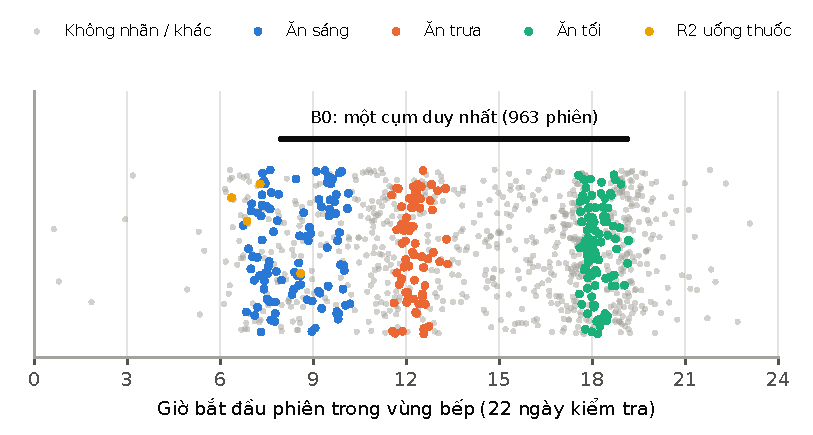
\includegraphics[width=\textwidth]{b0_kitchen_sessions}
\caption{Phiên trong vùng bếp của Cairo theo giờ bắt đầu (22 ngày kiểm tra), tô màu theo nhãn thật.
Phương pháp thực tập (B0) gộp toàn bộ thành một cụm duy nhất.}
\label{fig:b0}
\end{figure}

Ba bữa ăn tách bạch rõ ràng theo giờ, nhưng giữa chúng có rất nhiều phiên ngắn không nhãn --- hai người
đi lại xen kẽ khiến phiên bị cắt vụn (trung vị chỉ khoảng 2 phút). Các phiên này nối các bữa ăn lại với
nhau, và DBSCAN của phương pháp thực tập ``chuỗi hóa'' toàn bộ thành \textbf{một cụm 963 phiên trải từ
khoảng 8 giờ đến 19 giờ}. Thói quen uống thuốc của R2 --- chỉ vài phiên ngắn lẫn trong bữa sáng --- hoàn
toàn không thể tách ra. Đây không phải do thiếu nhãn mà là giới hạn của cách biểu diễn ``vùng × giờ''
khi trong nhà có hai người.

\section{RQ1 -- Nhận dạng (người, hoạt động)}
\label{sec:exp-rq1}

\begin{table}[htbp]
\centering
\caption{RQ1 -- F1 nhận dạng (người, hoạt động) theo sự kiện trên tập kiểm tra}
\label{tab:rq1}
\small
\begin{tabular}{lrrrrrr}
\toprule
Nhà & B2 macro-F1 & M1 macro-F1 & M2 macro-F1 & B2 micro-F1 & M1 micro-F1 & M2 micro-F1 \\
\midrule
Cairo & 0{,}32 & 0{,}41 & 0{,}38 & 0{,}49 & 0{,}57 & 0{,}40 \\
Tulum1 & 0{,}34 & 0{,}44 & 0{,}44 & 0{,}45 & 0{,}54 & 0{,}52 \\
Tulum2 & 0{,}40 & 0{,}48 & 0{,}46 & 0{,}49 & 0{,}57 & 0{,}55 \\
Milan & 0{,}35 & 0{,}49 & 0{,}47 & 0{,}59 & 0{,}69 & 0{,}67 \\
Aruba & 0{,}27 & 0{,}48 & 0{,}46 & 0{,}63 & 0{,}76 & 0{,}76 \\
\bottomrule
\end{tabular}
\end{table}


\begin{figure}[htbp]
\centering
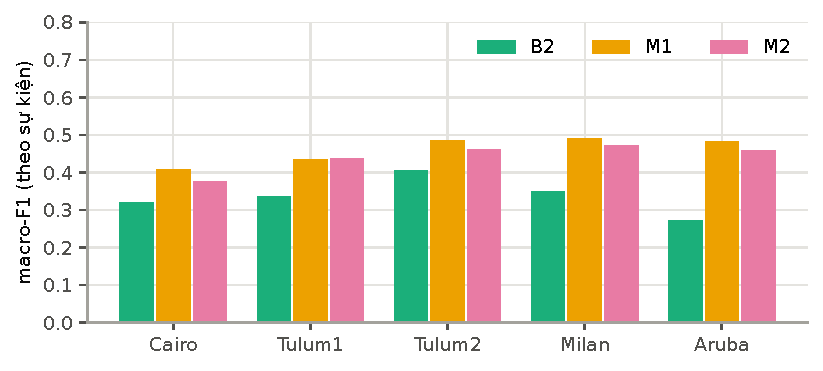
\includegraphics[width=0.85\textwidth]{rq1_macro_f1}
\caption{RQ1 -- macro-F1 theo sự kiện trên tập kiểm tra.}
\label{fig:rq1}
\end{figure}

Bảng~\ref{tab:rq1} và Hình~\ref{fig:rq1} cho thấy \textbf{hai mô hình học (M1, M2) vượt baseline tra
bảng B2 ở mọi nhà}, với chênh lệch macro-F1 từ 0,06 (Cairo, Tulum2) đến 0,21 (Aruba). M1 (Random
Forest) cao hơn M2 (Bi-GRU) ở bốn trên năm nhà; chỉ ở Tulum1 M2 nhỉnh hơn không đáng kể (0,438 so với
0,435). Mô hình chuỗi phức tạp hơn không mang lại lợi thế trên dữ liệu này --- phù hợp với việc Bi-GRU có
dấu hiệu học quá khớp ngay từ epoch thứ hai (Phụ lục~\ref{app:gru}).

Giá trị tuyệt đối (macro-F1 khoảng 0,38--0,49) thấp hơn nhiều so với các con số 80--90\% thường được báo
cáo trong tài liệu, kể cả trong~\cite{chen2021thesis}. Có ba lý do: (i) khóa luận \emph{chia theo thời
gian}, không xáo trộn; (ii) mỗi sự kiện được đánh giá với đầy đủ các hoạt động, kể cả các sự kiện không
thuộc hoạt động nào (chiếm phần lớn thời gian ở Cairo); (iii) Cairo, Tulum là nhà hai người với hoạt
động gắn người.

\begin{table}[htbp]
\centering
\caption{RQ1 -- F1 theo từng hoạt động trên Cairo}
\label{tab:rq1-cairo}
\small
\begin{tabular}{lrrr}
\toprule
Hoạt động & B2 & M1 & M2 \\
\midrule
Bed\_to\_Toilet & 0{,}30 & 0{,}16 & 0{,}22 \\
Breakfast & 0{,}42 & 0{,}51 & 0{,}57 \\
Dinner & 0{,}69 & 0{,}77 & 0{,}68 \\
Leave\_Home & 0{,}00 & 0{,}10 & 0{,}01 \\
Lunch & 0{,}55 & 0{,}65 & 0{,}60 \\
Night\_Wandering & 0{,}51 & 0{,}40 & 0{,}49 \\
R1\_Sleep & 0{,}05 & 0{,}35 & 0{,}30 \\
R1\_Wake & 0{,}35 & 0{,}56 & 0{,}46 \\
R1\_Work & 0{,}03 & 0{,}18 & 0{,}12 \\
R2\_Sleep & 0{,}49 & 0{,}41 & 0{,}42 \\
R2\_Take\_Medicine & 0{,}00 & 0{,}11 & 0{,}03 \\
R2\_Wake & 0{,}43 & 0{,}68 & 0{,}61 \\
\bottomrule
\end{tabular}
\end{table}


Bảng~\ref{tab:rq1-cairo} chi tiết theo hoạt động trên Cairo. Các bữa ăn và thức dậy đạt F1 0,5--0,8.
\textbf{Uống thuốc của R2 chỉ đạt 0,11} với M1: đây là hoạt động rất ngắn (trung vị 1,2 phút), diễn ra
ở đúng cảm biến bếp và cùng khung giờ với bữa sáng. ``Rời nhà'' (\texttt{Leave\_Home}) gần như không
nhận ra được vì hầu như không có sự kiện chuyển động nào trong lúc vắng nhà.

\section{RQ2 -- Thói quen của từng người}
\label{sec:exp-rq2}

\begin{table}[htbp]
\centering
\caption{RQ2 -- F1 thói quen theo nhà và phương pháp}
\label{tab:rq2-f1}
\small
\begin{tabular}{lrrrrrr}
\toprule
Phương pháp & Cairo & Tulum1 & Tulum2 & Milan & Aruba & Trung bình \\
\midrule
B0 & 0{,}24 & 0{,}22 & 0{,}33 & 0{,}38 & 0{,}29 & 0{,}29 \\
B1 & 0{,}12 & 0{,}22 & 0{,}18 & 0{,}38 & 0{,}27 & 0{,}23 \\
B2+H & 0{,}43 & 0{,}59 & 0{,}54 & 0{,}40 & 0{,}63 & 0{,}52 \\
M1+H & 0{,}62 & 0{,}71 & 0{,}50 & 0{,}54 & 0{,}59 & 0{,}59 \\
M2+H & 0{,}37 & 0{,}75 & 0{,}51 & 0{,}55 & 0{,}50 & 0{,}54 \\
Oracle+H & 1{,}00 & 1{,}00 & 1{,}00 & 1{,}00 & 1{,}00 & 1{,}00 \\
\bottomrule
\end{tabular}
\end{table}


\begin{figure}[htbp]
\centering
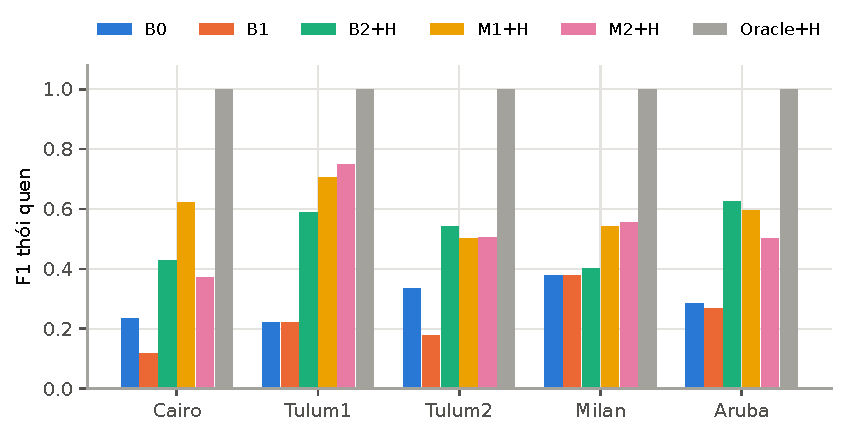
\includegraphics[width=\textwidth]{rq2_habit_f1}
\caption{RQ2 -- F1 của thói quen tìm được so với thói quen đáp án.}
\label{fig:rq2}
\end{figure}

Bảng~\ref{tab:rq2-f1} và Hình~\ref{fig:rq2} là kết quả trung tâm của khóa luận.

\textbf{(1) Học (người, hoạt động) rồi áp định nghĩa thói quen tốt hơn hẳn phương pháp theo vùng.} Trên
cả ba nhà hai người, M1+H đạt F1 thói quen 0,50--0,71 (M2+H: 0,37--0,75), trong khi B0 chỉ đạt
0,22--0,33. Khác biệt
nằm chủ yếu ở \emph{recall}: B0 tìm được rất ít thói quen có nghĩa (recall 0,17--0,22) vì các thói quen
bị gộp như mục~\ref{sec:exp-b0}.

\textbf{(2) Thói quen từng người ở Cairo.} Bảng~\ref{tab:rq2-cairo} và Hình~\ref{fig:timeline} chi tiết
Cairo. \textbf{M1+H tìm được đủ 6/6 thói quen gắn người}, trong đó có ``R2 uống thuốc 06:57'' (đáp án
07:08, ngày thường) --- đúng ví dụ mở đầu khóa luận. B0 chỉ tìm được 2/6, với khung giờ rộng hàng chục
giờ.

\begin{table}[htbp]
\centering
\caption{RQ2 -- So khớp thói quen với đáp án trên Cairo}
\label{tab:rq2-cairo}
\small
\begin{tabular}{lrrrrcc}
\toprule
Phương pháp & P & R & F1 & Lệch giờ (phút) & Khớp/đáp án & Từng người \\
\midrule
B0 & 0{,}25 & 0{,}22 & 0{,}24 & 32{,}03 & 2/9 & 2/6 \\
B1 & 0{,}13 & 0{,}11 & 0{,}12 & 31{,}49 & 1/9 & 0/6 \\
B2+H & 0{,}32 & 0{,}67 & 0{,}43 & 29{,}97 & 6/9 & 3/6 \\
M1+H & 0{,}45 & 1{,}00 & 0{,}62 & 13{,}19 & 9/9 & 6/6 \\
M2+H & 0{,}24 & 0{,}89 & 0{,}37 & 22{,}17 & 8/9 & 5/6 \\
Oracle+H & 1{,}00 & 1{,}00 & 1{,}00 & 0{,}00 & 9/9 & 6/6 \\
\bottomrule
\end{tabular}
\end{table}


\begin{figure}[htbp]
\centering
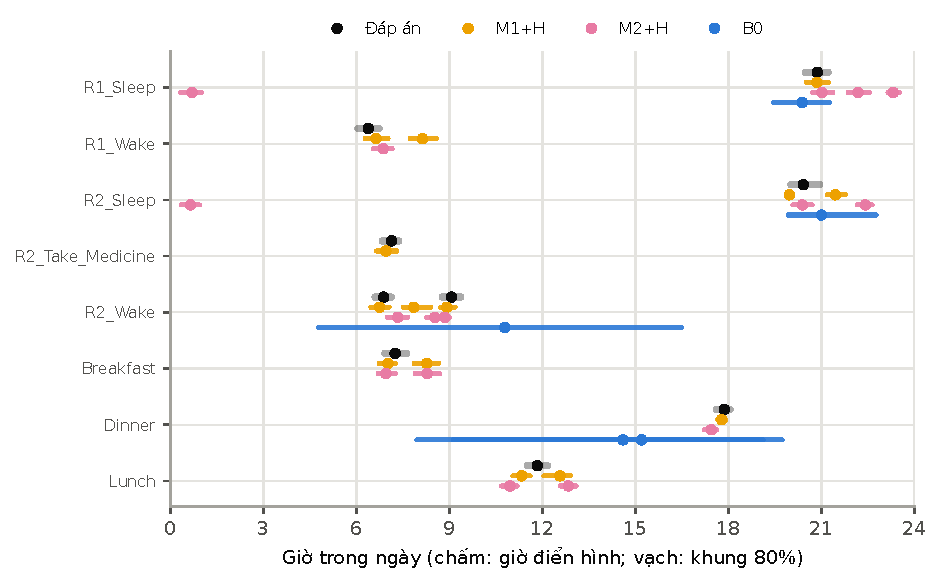
\includegraphics[width=\textwidth]{habits_timeline_cairo}
\caption{Thói quen trên Cairo: đáp án (đen), M1+H, M2+H và B0. Chấm là giờ điển hình, vạch là khung 80\%.}
\label{fig:timeline}
\end{figure}

\textbf{(3) Tách vệt theo vị trí (B1) không giúp, thậm chí làm tệ hơn.} Ở Cairo, B1 đạt 0,12 so với 0,24
của B0; ở Tulum2 là 0,18 so với 0,33. Heuristic ``sự kiện xa nhau thuộc hai người'' cắt vụn thêm các
phiên (số phiên tăng từ 2.748 lên 4.219 ở Cairo) mà không gắn được phiên với \emph{người cụ thể}: hai vệt
là vô danh và có thể đổi vai cho nhau theo thời gian. Kết quả này cho thấy, ít nhất với cảm biến chuyển
động thưa, \emph{tách người không cần nhãn} chưa đủ để học thói quen từng người; cần một tín hiệu học có
giám sát như ở M1, M2.

\textbf{(4) Khi thói quen chủ yếu gắn với ``vùng + giờ'', tra bảng đã khá tốt.} Ở Tulum2, B2+H (0,54)
ngang M1+H (0,50) và M2+H (0,51); ở Aruba (nhà một người), B2+H còn cao nhất (0,63 so với 0,59 của
M1+H). Phần lớn thói quen của Tulum2 là hoạt động chung lặp lại nhiều lần trong ngày (vệ sinh, xem
TV, làm việc), gắn chặt với ``vùng nào, khung giờ nào''. Ưu thế của mô hình học thể hiện rõ nhất ở các
hoạt động gắn người và hoạt động ngắn, như ở Cairo.

\textbf{(5) Lỗi chính của mô hình học là thói quen giả, không phải bỏ sót.} Ở mọi nhà, recall của M1+H và
M2+H cao (0,68--1,00) nhưng precision chỉ khoảng 0,24--0,60. Bảng~\ref{tab:false-cairo} truy ngược 11 thói
quen giả của M1+H trên Cairo: với mỗi thói quen giả, các lần thực hiện tạo nên nó được đối chiếu với nhãn
thật trùng thời gian. Hai nguồn lỗi hiện ra rõ:
\begin{itemize}
  \item \emph{Thói quen ``lệch bóng''} nằm ngay cạnh một thói quen thật của cùng hoạt động (ăn sáng 08:16
  cạnh 07:15; ăn trưa 12:34 cạnh 11:50; R2 thức dậy 07:51 cạnh 06:53; R2 ngủ 21:27 cạnh 20:25): bộ nhận dạng
  tiếp tục báo hoạt động sau khi nó đã kết thúc, đều đặn mỗi ngày, nên phần ``đuôi'' này tự thành một thói
  quen thứ hai.
  \item \emph{Khoảng không có nhãn}: ở 8/11 thói quen giả (kể cả phần lớn các thói quen lệch bóng ở trên),
  đa số các lần thực hiện rơi vào khoảng thời gian không có nhãn nào. Cairo chỉ được gán nhãn khoảng 2,5 giờ mỗi ngày, nên một phần các thói quen này có thể
  là hoạt động thật mà người chú thích không ghi (ví dụ các lần ``rời nhà'' 09:41, 13:01, 15:15).
\end{itemize}
Chỉ một trường hợp là nhầm hoạt động rõ ràng (``R1 làm việc 21:26'' trùng giờ R1 đi ngủ). Cả hai nguồn lỗi
chính đều là lỗi \emph{có hệ thống} --- lặp lại cùng một kiểu, cùng một giờ, ngày nào cũng như ngày nào ---
nên đủ nhiều để vượt ngưỡng 50\% số ngày. Mục~\ref{sec:exp-prop} sẽ cho thấy lỗi \emph{ngẫu nhiên} thì gần
như vô hại.

\begin{table}[htbp]
\centering
\caption{Thói quen giả của M1+H trên Cairo: mỗi dòng truy các lần thực hiện tạo nên thói quen về nhãn thật trùng thời gian}
\label{tab:false-cairo}
\small
\begin{tabular}{lccl}
\toprule
Thói quen giả & Số ngày & Thói quen thật gần nhất & Nhãn thật trùng nhiều nhất \\
\midrule
Ăn sáng 08:16 & 15 & 07:15 (lệch 61 phút) & (không nhãn) (11/18) \\
Rời nhà 09:41 & 4 & không có & (không nhãn) (6/9) \\
Rời nhà 13:01 & 4 & không có & (không nhãn) (7/8) \\
Rời nhà 15:15 & 4 & không có & (không nhãn) (5/5) \\
Ăn trưa 12:34 & 13 & 11:50 (lệch 44 phút) & (không nhãn) (10/14) \\
Đi lại ban đêm 00:56 & 14 & không có & (không nhãn) (7/16) \\
Đi lại ban đêm 03:50 & 16 & không có & Đi lại ban đêm (7/17) \\
R1 thức dậy 08:08 & 11 & 06:23 (lệch 105 phút) & R1 thức dậy (5/12) \\
R1 làm việc 21:26 & 4 & không có & R1 ngủ (4/11) \\
R2 ngủ 21:27 & 16 & 20:25 (lệch 61 phút) & (không nhãn) (13/21) \\
R2 thức dậy 07:51 & 12 & 06:53 (lệch 59 phút) & (không nhãn) (7/13) \\
\bottomrule
\end{tabular}
\end{table}


\textbf{(6) B0 bảo thủ: ít sai nhưng bỏ sót nhiều.} Ở Milan, Aruba và Tulum2, những thói quen B0 tìm ra
phần lớn là đúng (precision 0,64--0,75), nhưng nó chỉ tìm được 18--27\% số thói quen đáp án. Ở Cairo và
Tulum1 --- hai nhà mà hoạt động của hai người chồng lấn mạnh trong cùng vùng bếp --- precision của B0 cũng
giảm còn 0,25--0,33. Ngay ở nhà một người, M1+H và M2+H vẫn vượt B0 (0,50--0,59 so với 0,29--0,38): đơn
vị ``phiên trong vùng'' quá thô cho thói quen gắn với \emph{hoạt động}.

\section{Phân tích lỗi lan truyền}
\label{sec:exp-prop}

\begin{figure}[htbp]
\centering
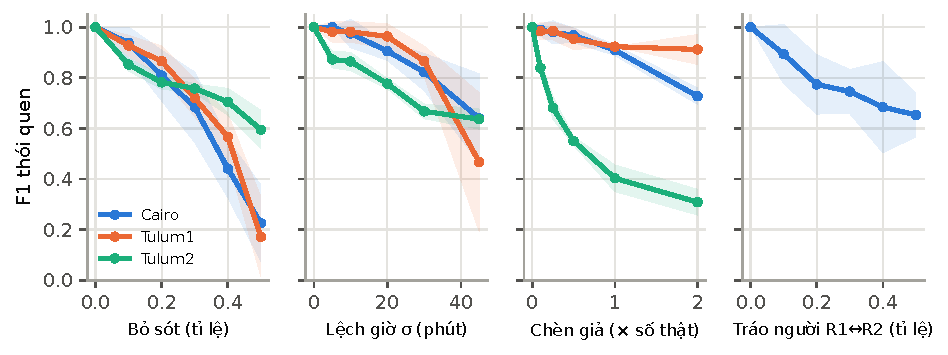
\includegraphics[width=\textwidth]{propagation}
\caption{F1 thói quen khi làm nhiễu nhãn thật có kiểm soát (trung bình $\pm$ độ lệch chuẩn qua 5 hạt
giống). Đường ``tráo người'' chỉ vẽ cho nhà có ít nhất 3 thói quen gắn người (Cairo).}
\label{fig:prop}
\end{figure}

Hình~\ref{fig:prop} trả lời phần thứ hai của RQ2: \emph{nhận dạng sai bao nhiêu thì thói quen sai bấy
nhiêu?}

\begin{itemize}
  \item \textbf{Bỏ sót là nguy hiểm nhất.} Vì thói quen cần xuất hiện ở ít nhất 50\% số ngày, bỏ sót đẩy
  tần suất xuống dưới ngưỡng. Ở Cairo, bỏ sót 20\% số lần thực hiện làm F1 còn 0,81; bỏ sót 40\% còn 0,44.
  \item \textbf{Lệch giờ gần như vô hại khi nhỏ.} Lệch chuẩn 10 phút giữ F1 ở 0,98 (Cairo); chỉ khi lệch
  từ 30 phút trở lên --- bằng nửa bề rộng cửa sổ --- F1 mới giảm rõ.
  \item \textbf{Chèn giả ngẫu nhiên ít ảnh hưởng}, đến khi số lần giả bằng số lần thật (Cairo: 0,91). Lỗi
  ngẫu nhiên rải đều trong ngày nên không tạo được đỉnh đạt 50\% số ngày. Đối chiếu với kết quả (5) ở
  mục~\ref{sec:exp-rq2}: \emph{lỗi có hệ thống} của bộ nhận dạng mới sinh thói quen giả.
  \item \textbf{Tráo người} R1$\leftrightarrow$R2 với xác suất 20\% làm F1 thói quen gắn người của Cairo
  còn 0,77. Một thói quen gắn người chịu được mức nhầm người vừa phải vì lần thực hiện đúng người vẫn
  chiếm đa số, nhưng thói quen sát ngưỡng bị mất trước.
  \item \textbf{Độ bền phụ thuộc khoảng cách tới ngưỡng.} Tulum2 nhạy hơn hẳn Cairo với mọi loại lỗi
  (chèn giả 10\% đã còn 0,84): thói quen của Tulum2 là các hoạt động lặp nhiều lần với tần suất chỉ vừa
  qua 50\%, nên một chút nhiễu đủ đẩy chúng qua lại ngưỡng.
\end{itemize}

\textbf{Hàm ý thực tế.} Để học thói quen, một bộ nhận dạng cần ưu tiên \emph{không bỏ sót} và \emph{không
nhầm có hệ thống}; sai lệch giờ nhỏ và nhận thừa rải rác là chấp nhận được. Điều này khác với tiêu chí
accuracy/F1 theo sự kiện thường dùng để tối ưu mô hình nhận dạng.

\section{Ablation và độ nhạy}
\label{sec:exp-ablation}

\begin{table}[htbp]
\centering
\caption{Ablation -- F1 thói quen khi thay một thành phần (dòng ``Nhãn thật'': khai phá trên nhãn thật của ngày kiểm tra)}
\label{tab:ablation}
\small
\begin{tabular}{llrrrrr}
\toprule
Đầu vào & Biến thể & Cairo & Tulum1 & Tulum2 & Milan & Aruba \\
\midrule
Nhãn thật & Quét cửa sổ (mặc định) & 1{,}00 & 1{,}00 & 1{,}00 & 1{,}00 & 1{,}00 \\
Nhãn thật & DBSCAN & 0{,}90 & 0{,}92 & 0{,}63 & 0{,}77 & 0{,}38 \\
Nhãn thật & HDBSCAN & 0{,}61 & 0{,}22 & 0{,}50 & 0{,}75 & 0{,}52 \\
Nhãn thật & Không tách loại ngày & 0{,}71 & 1{,}00 & 0{,}56 & 0{,}79 & 0{,}71 \\
\midrule
M1 & Mặc định (quét cửa sổ, nối 10 phút) & 0{,}62 & 0{,}71 & 0{,}50 & 0{,}54 & 0{,}59 \\
M1 & DBSCAN & 0{,}64 & 0{,}53 & 0{,}51 & 0{,}52 & 0{,}08 \\
M1 & HDBSCAN & 0{,}41 & 0{,}53 & 0{,}37 & 0{,}60 & 0{,}53 \\
M1 & Không tách loại ngày & 0{,}67 & 0{,}71 & 0{,}49 & 0{,}54 & 0{,}50 \\
\midrule
M1 & Khoảng nối 2 phút & 0{,}69 & 0{,}71 & 0{,}61 & 0{,}56 & 0{,}38 \\
M1 & Khoảng nối 5 phút & 0{,}64 & 0{,}75 & 0{,}60 & 0{,}53 & 0{,}45 \\
M1 & Khoảng nối 20 phút & 0{,}67 & 0{,}71 & 0{,}47 & 0{,}61 & 0{,}32 \\
M1 & Khoảng nối 30 phút & 0{,}62 & 0{,}75 & 0{,}43 & 0{,}68 & 0{,}33 \\
\bottomrule
\end{tabular}
\end{table}


\textbf{Thuật toán khai phá.} Trên nhãn thật (dòng ``Oracle''), DBSCAN chỉ khớp định nghĩa ở mức F1
0,38--0,92 và HDBSCAN ở mức 0,22--0,75 tùy nhà: DBSCAN chuỗi hóa các hoạt động lặp nhiều lần (chỉ còn 0,38
ở Aruba), HDBSCAN không có khái niệm ``lệch không quá 30 phút''. Đây là căn cứ để khóa luận hiện thực định
nghĩa bằng thuật toán quét cửa sổ thay vì HDBSCAN như dự kiến ban đầu. Trên đầu ra của M1, quét cửa sổ tốt
nhất ở Tulum1 và Aruba (DBSCAN chỉ còn 0,08 ở Aruba), chênh không quá 0,02 so với DBSCAN ở Cairo, Milan và
Tulum2; HDBSCAN cao hơn ở Milan (0,60 so với 0,54) nhưng thấp hơn rõ ở Cairo và Tulum2. Ưu điểm chính của
quét cửa sổ là \emph{đúng định nghĩa} và \emph{không sụp} ở bất kỳ nhà nào.

\textbf{Tách ngày thường -- cuối tuần.} Kết quả lẫn lộn: bỏ bước này làm F1 của M1 giảm ở Aruba (0,59
$\rightarrow$ 0,50), tăng ở Cairo (0,62 $\rightarrow$ 0,67) và gần như không đổi ở ba nhà còn lại. Với số
ngày kiểm tra ít (6--16 ngày cuối tuần ở các nhà nhỏ), thói quen riêng cuối tuần dễ là thói quen giả; với
nhà có nhiều ngày như Aruba (88 ngày kiểm tra), bước này giúp ích. Bước này hữu ích khi đáp án có thói quen riêng cuối tuần rõ ràng (``R2 dậy
muộn 9:04 cuối tuần'' ở Cairo) nhưng cần nhiều ngày hơn để ổn định.

\textbf{Khoảng nối khi giải mã.} Khoảng nối là tham số nhạy: ở Aruba, F1 của M1 dao động 0,32--0,59 (tốt nhất
ở 10 phút); ở các nhà khác dao động đến 0,2 và không có giá trị tốt nhất chung (Tulum2 thích khoảng ngắn,
Milan thích khoảng dài). Đây là điểm cần cải tiến: bước giải mã nên xét thời lượng điển hình của từng hoạt
động thay vì một khoảng nối chung.

\begin{table}[htbp]
\centering
\caption{Độ nhạy -- F1 thói quen trung bình năm nhà khi đổi tham số định nghĩa}
\label{tab:sensitivity}
\small
\begin{tabular}{rrrrrrr}
\toprule
Cửa sổ $\pm$(phút) & Ngưỡng & B0 & B1 & B2+H & M1+H & M2+H \\
\midrule
15 & 0{,}40 & 0{,}26 & 0{,}20 & 0{,}43 & 0{,}50 & 0{,}46 \\
15 & 0{,}50 & 0{,}28 & 0{,}26 & 0{,}32 & 0{,}38 & 0{,}35 \\
15 & 0{,}60 & 0{,}19 & 0{,}19 & 0{,}35 & 0{,}33 & 0{,}35 \\
30 & 0{,}40 & 0{,}28 & 0{,}23 & 0{,}51 & 0{,}64 & 0{,}57 \\
30 & 0{,}50 & 0{,}29 & 0{,}23 & 0{,}52 & 0{,}59 & 0{,}54 \\
30 & 0{,}60 & 0{,}28 & 0{,}22 & 0{,}44 & 0{,}52 & 0{,}44 \\
45 & 0{,}40 & 0{,}31 & 0{,}26 & 0{,}50 & 0{,}61 & 0{,}55 \\
45 & 0{,}50 & 0{,}31 & 0{,}25 & 0{,}54 & 0{,}64 & 0{,}59 \\
45 & 0{,}60 & 0{,}30 & 0{,}22 & 0{,}53 & 0{,}58 & 0{,}52 \\
\bottomrule
\end{tabular}
\end{table}


\textbf{Độ nhạy theo định nghĩa.} Bảng~\ref{tab:sensitivity} thay đồng thời tham số của định nghĩa cho cả
đáp án và dự đoán. Với cửa sổ $\pm 30$ và $\pm 45$ phút, thứ tự trung bình các phương pháp ổn định: M1+H $>$ M2+H $\approx$
B2+H $>$ B0 $>$ B1. Với cửa sổ hẹp $\pm 15$ phút, mọi phương pháp giảm mạnh và khoảng cách giữa mô hình học
và tra bảng gần như biến mất ---
cửa sổ hẹp hơn sai số giờ bắt đầu của bộ nhận dạng. Định nghĩa $\pm 30$ phút là điểm cân bằng hợp lý giữa
``đủ chặt để có nghĩa'' và ``đủ rộng để học được''.

\section{RQ3 -- Phát hiện ngày bỏ thuốc}
\label{sec:exp-rq3}

\begin{table}[htbp]
\centering
\caption{RQ3 -- Phát hiện ngày bỏ thuốc \texttt{R2\_Take\_Medicine} trên Cairo (trung bình 5 lần cài; F1 ghi trung bình $\pm$ độ lệch chuẩn)}
\label{tab:rq3}
\small
\begin{tabular}{lrrcr}
\toprule
Bộ phát hiện & P & R & F1 & Báo nhầm/ngày \\
\midrule
B0-vùng & 0{,}00 & 0{,}00 & 0{,}00 $\pm$ 0{,}00 & 0{,}00 \\
B2 & 0{,}20 & 1{,}00 & 0{,}33 $\pm$ 0{,}00 & 0{,}80 \\
M1 & 0{,}00 & 0{,}00 & 0{,}00 $\pm$ 0{,}00 & 0{,}00 \\
M2 & 0{,}25 & 0{,}90 & 0{,}39 $\pm$ 0{,}10 & 0{,}54 \\
\bottomrule
\end{tabular}
\end{table}


\begin{figure}[htbp]
\centering
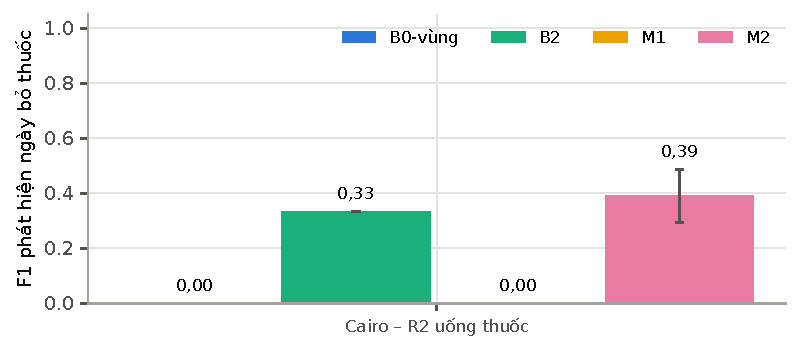
\includegraphics[width=0.75\textwidth]{rq3_detection}
\caption{RQ3 -- F1 phát hiện ngày bỏ thuốc trên Cairo (trung bình $\pm$ độ lệch chuẩn qua 5 lần cài).}
\label{fig:rq3}
\end{figure}

\textbf{Thiết lập thực tế.} Thói quen chuẩn ``R2 uống thuốc'' học từ ngày huấn luyện có cửa sổ phát hiện
06:19--07:58. Trong 22 ngày kiểm tra của Cairo, \textbf{12 ngày không có nhãn uống thuốc nào trong cửa
sổ} --- không thể biết R2 bỏ thuốc thật hay người chú thích không ghi. Những ngày này bị loại khỏi chấm
điểm, còn 10 ngày; mỗi lần cài chọn 2 ngày làm ngày bỏ thuốc. Ở Milan, giờ uống thuốc trong giai đoạn huấn
luyện dao động quá rộng (thuốc sáng khoảng 08:06--10:25; thuốc tối chỉ có nhãn 5/37 ngày) nên không tạo
được thói quen chuẩn theo định nghĩa; RQ3 vì vậy chỉ đánh giá được trên Cairo.

\textbf{Kết quả} (Bảng~\ref{tab:rq3}, Hình~\ref{fig:rq3}):
\begin{itemize}
  \item \textbf{B0-vùng và M1 không bao giờ báo động.} Khi xóa sự kiện uống thuốc, vùng bếp vẫn có người
  (bữa sáng), nên B0-vùng luôn thấy ``bình thường''. M1 cũng vẫn ``thấy'' uống thuốc: Random Forest học
  ngữ cảnh ``bếp, khoảng 7 giờ'' chứ không học dấu hiệu riêng của việc uống thuốc. Đây chính là lỗi có
  hệ thống đã nói ở mục~\ref{sec:exp-rq2}.
  \item \textbf{M2 phát hiện 9/10 ngày bỏ thuốc} (tổng qua 5 lần cài; recall 0,90) nhưng báo động nhầm
  0,54 lần mỗi ngày.
  Mô hình chuỗi nhạy hơn với việc thiếu một đoạn sự kiện ngắn, đổi lại kém ổn định.
  \item B2 báo động gần như mọi ngày (recall 1,0, precision 0,2) nên không có giá trị sử dụng.
\end{itemize}
Vì bộ phát hiện chờ hết cửa sổ (07:58) mới kết luận, báo động đến khoảng 47 phút sau giờ uống thuốc điển
hình --- đủ sớm để nhắc trong cùng buổi sáng.

\textbf{Nhận định.} RQ3 cho câu trả lời \emph{một phần}: thói quen học được \emph{có} chứa thông tin để
phát hiện bỏ thuốc (M2), và tốt hơn hẳn cách theo vùng (vốn không thể phát hiện), nhưng chưa đủ tin cậy
để dùng thực tế: số báo động nhầm còn cao và mẫu đánh giá nhỏ (10 ngày dương tính qua 5 lần cài). Kết
quả này cũng cho thấy một điểm đáng chú ý: \emph{mô hình tốt hơn ở RQ2 (M1) lại kém hơn ở RQ3}, vì phát
hiện ``vắng mặt'' đòi hỏi mô hình dựa vào dấu hiệu riêng của hoạt động chứ không dựa vào ngữ cảnh.

\section{Thảo luận}
\label{sec:exp-discussion}

\textbf{Trả lời ba câu hỏi nghiên cứu.}
\begin{description}[leftmargin=1.2cm,style=sameline]
  \item[RQ1] Gán (người, hoạt động) theo sự kiện đạt macro-F1 khoảng 0,38--0,49 với mô hình học khi đánh
  giá theo thời gian; mô hình học vượt tra bảng ở mọi nhà. Hoạt động ngắn, trùng chỗ (uống thuốc) và hoạt
  động ít sự kiện (rời nhà) là khó nhất.
  \item[RQ2] Dù nhận dạng theo sự kiện còn thấp, thói quen tìm được vẫn tốt hơn hẳn phương pháp theo vùng:
  F1 0,50--0,71 (M1+H) so với 0,22--0,33 ở nhà hai người, và đủ 6/6 thói quen gắn người ở Cairo. Thói quen
  \emph{chịu được} lệch giờ nhỏ và nhận thừa ngẫu nhiên, nhưng \emph{nhạy} với bỏ sót, nhầm người và lỗi
  có hệ thống.
  \item[RQ3] Có thể phát hiện ngày bỏ thuốc ở mức nhất định (M2: recall 0,9), nhưng báo động nhầm còn cao;
  cách theo vùng hoàn toàn không phát hiện được.
\end{description}

\textbf{Mối đe dọa tính hợp lệ.}
\begin{itemize}
  \item \emph{Số thói quen gắn người nhỏ} (6 ở Cairo, 1 ở mỗi nhà Tulum): kết luận về ``từng người'' chủ
  yếu dựa trên Cairo.
  \item \emph{Nhãn thưa}: Cairo chỉ gán nhãn khoảng 2,5 giờ mỗi ngày; một thói quen ``giả'' có thể là thói
  quen thật mà người chú thích không ghi.
  \item \emph{Một lần chia dữ liệu}: kết quả dựa trên một lần chia 60/40 theo thời gian; chưa có khoảng tin
  cậy theo nhiều lần chia (dự kiến bổ sung ở bản v2).
  \item \emph{Gán nhãn cho cụm B0, B1 dùng nhãn tập kiểm tra}: có lợi cho baseline; so sánh vì thế thận trọng.
  \item \emph{Bất thường được cài}: ngày bỏ thuốc thật có thể để lại dấu vết khác (ví dụ không mở tủ thuốc
  nhưng vẫn vào bếp lâu hơn).
\end{itemize}
